% !TEX root = ../main.tex
% Measurement setups (I-U, P-I, spectral), redrawn in TikZ.
% Include with % !TEX root = ../main.tex
% Measurement setups (I-U, P-I, spectral), redrawn in TikZ.
% Include with % !TEX root = ../main.tex
% Measurement setups (I-U, P-I, spectral), redrawn in TikZ.
% Include with % !TEX root = ../main.tex
% Measurement setups (I-U, P-I, spectral), redrawn in TikZ.
% Include with \input{chapters/measurement_setup.tex}; reference the whole figure
% with \cref{fig:setup} or a single setup with \cref{fig:setup_iu},
% \cref{fig:setup_pi} and \cref{fig:setup_spectral}.

\tikzset{
	setup/.style={font=\small, line width=0.6pt},
	meter/.style={circle, draw, fill=white, minimum size=0.75cm, inner sep=0pt},
	% instrument box with display; terminals (-a) left and (-b) right, origin at (-b)
	instrument/.pic={
		\draw (-2.8,-0.35) rectangle (0.25,1.0);
		\node[draw, rounded corners=2pt, anchor=north west, minimum width=1.2cm,
			minimum height=0.4cm, inner sep=2pt] at (-2.65,0.85) {#1};
		\fill (-0.25,0) circle (2pt) coordinate (-a);
		\fill (0,0) circle (2pt) coordinate (-b);
	},
	ground/.pic={
		\draw (0,0) -- (0,-0.9);
		\draw[line width=1.4pt] (-0.3,-0.9) -- (0.3,-0.9);
	},
	% laser diode pointing to the right, centred at the origin
	diode/.pic={
		\fill (-0.18,0.2) -- (-0.18,-0.2) -- (0.18,0) -- cycle;
		\draw[line width=1.2pt] (0.18,0.2) -- (0.18,-0.2);
	},
	emission/.pic={
		\draw[-{Stealth[length=4pt]}] (-0.15,0.3) -- (0.2,0.7);
		\draw[-{Stealth[length=4pt]}] (0.05,0.3) -- (0.4,0.7);
	},
	% temperature-controlled mount below the diode
	mount/.pic={
		\draw[fill=gray!30] (-0.12,-0.25) rectangle (0.12,-1.0);
		\draw[fill=gray!60] (-0.3,-1.0) rectangle (0.3,-1.15);
	},
}

\begin{figure}[H]
	\centering
	\begin{subfigure}{\linewidth}
		\centering
		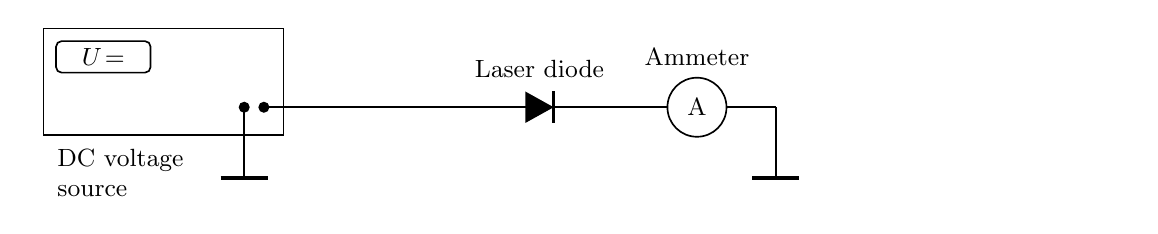
\begin{tikzpicture}[setup]
			\path (-3,0) -- (11,0);
			\pic (src) at (0,0) {instrument={$U\!=$}};
			\node[anchor=north west, align=left] at (-2.75,-0.4) {DC voltage\\source};
			\pic at (src-a) {ground};
			\draw (src-b) -- (6.5,0);
			\pic at (3.5,0) {diode};
			\node[above] at (3.5,0.25) {Laser diode};
			\node[meter] at (5.5,0) {A};
			\node[above] at (5.5,0.4) {Ammeter};
			\pic at (6.5,0) {ground};
		\end{tikzpicture}
		\caption{Current-voltage characteristic.}
		\label{fig:setup_iu}
	\end{subfigure}

	\vspace{0.6cm}
	\begin{subfigure}{\linewidth}
		\centering
		\begin{tikzpicture}[setup]
			\path (-3,0) -- (11,0);
			\pic (gen) at (0,0) {instrument={$I\!=$}};
			\node[anchor=north west, align=left] at (-2.75,-0.4) {Pulse\\generator};
			\pic at (gen-a) {ground};
			\draw (gen-b) -- (5.9,0);
			\draw (0.6,0.15) -- (0.9,0.15) -- (0.9,0.6) -- (1.2,0.6) -- (1.2,0.15) -- (1.5,0.15);
			% voltage measurement at the diode
			\fill (2.2,0) circle (2pt);
			\node[meter] (V) at (2.2,-1.0) {U};
			\draw (2.2,0) -- (V);
			\pic at (V.south) {ground};
			% laser diode on mount with detector
			\pic at (3.6,0) {mount};
			\pic at (3.6,0) {diode};
			\pic at (3.6,0) {emission};
			\draw (4.3,0.8) rectangle (5.5,1.1);
			\node[above] at (4.9,1.1) {Detector};
			\node[meter] at (5.1,0) {A};
			\pic at (5.9,0) {ground};
			% lock-in amplifier
			\pic (lock) at (10.5,0) {instrument={Lock-in}};
			\draw (5.5,0.95) -- (6.8,0.95) -- (6.8,-0.6) -- (10.25,-0.6) -- (lock-a);
			\pic at (lock-b) {ground};
		\end{tikzpicture}
		\caption{Optical power-current characteristic.}
		\label{fig:setup_pi}
	\end{subfigure}

	\vspace{0.6cm}
	\begin{subfigure}{\linewidth}
		\centering
		\begin{tikzpicture}[setup]
			\path (-3,0) -- (11,0);
			\pic (src) at (0,0) {instrument={$I\!=$}};
			\node[anchor=north west, align=left] at (-2.75,-0.4) {DC current\\source};
			\pic at (src-a) {ground};
			\draw (src-b) -- (5.3,0);
			\pic at (3.2,0) {mount};
			\pic at (3.2,0) {diode};
			\pic at (3.2,0) {emission};
			\node[meter] at (4.5,0) {A};
			\pic at (5.3,0) {ground};
			% lens focusing onto the monochromator entrance slit
			\draw (4.0,1.25) ellipse (0.12 and 0.42);
			\draw (4.1,1.6) -- (6.0,1.25) -- (4.1,0.9);
			\draw (6.0,0.6) rectangle (9.2,1.9);
			\node[anchor=south east] at (9.2,0.6) {Monochromator};
			\draw (9.2,1.3) rectangle (10.3,1.9);
			\node at (9.75,1.6) {PMT};
			% computer
			\draw[rounded corners=2pt] (7.9,-1.05) rectangle (9.1,0.05);
			\draw[rounded corners=1pt] (8.05,-0.9) rectangle (8.95,-0.1);
			\draw (8.3,-1.05) -- (8.2,-1.3) -- (8.8,-1.3) -- (8.7,-1.05);
			\draw (7.6,-1.3) rectangle (9.6,-1.85);
			\foreach \x in {7.75,7.85,...,8.45} \draw (\x,-1.42) -- (\x,-1.73);
			\draw (8.9,-1.5) rectangle (9.4,-1.65);
			\draw (9.75,1.3) .. controls (9.9,0.0) and (10.1,-1.4) .. (9.6,-1.55);
		\end{tikzpicture}
		\caption{Spectral measurements.}
		\label{fig:setup_spectral}
	\end{subfigure}
	\caption{Measurement setups for the characterisation of the laser diode. The diode
	is placed on a temperature-controlled mount for the P-I and spectral measurements.
	PMT: photomultiplier tube.}
	\label{fig:setup}
\end{figure}
; reference the whole figure
% with \cref{fig:setup} or a single setup with \cref{fig:setup_iu},
% \cref{fig:setup_pi} and \cref{fig:setup_spectral}.

\tikzset{
	setup/.style={font=\small, line width=0.6pt},
	meter/.style={circle, draw, fill=white, minimum size=0.75cm, inner sep=0pt},
	% instrument box with display; terminals (-a) left and (-b) right, origin at (-b)
	instrument/.pic={
		\draw (-2.8,-0.35) rectangle (0.25,1.0);
		\node[draw, rounded corners=2pt, anchor=north west, minimum width=1.2cm,
			minimum height=0.4cm, inner sep=2pt] at (-2.65,0.85) {#1};
		\fill (-0.25,0) circle (2pt) coordinate (-a);
		\fill (0,0) circle (2pt) coordinate (-b);
	},
	ground/.pic={
		\draw (0,0) -- (0,-0.9);
		\draw[line width=1.4pt] (-0.3,-0.9) -- (0.3,-0.9);
	},
	% laser diode pointing to the right, centred at the origin
	diode/.pic={
		\fill (-0.18,0.2) -- (-0.18,-0.2) -- (0.18,0) -- cycle;
		\draw[line width=1.2pt] (0.18,0.2) -- (0.18,-0.2);
	},
	emission/.pic={
		\draw[-{Stealth[length=4pt]}] (-0.15,0.3) -- (0.2,0.7);
		\draw[-{Stealth[length=4pt]}] (0.05,0.3) -- (0.4,0.7);
	},
	% temperature-controlled mount below the diode
	mount/.pic={
		\draw[fill=gray!30] (-0.12,-0.25) rectangle (0.12,-1.0);
		\draw[fill=gray!60] (-0.3,-1.0) rectangle (0.3,-1.15);
	},
}

\begin{figure}[H]
	\centering
	\begin{subfigure}{\linewidth}
		\centering
		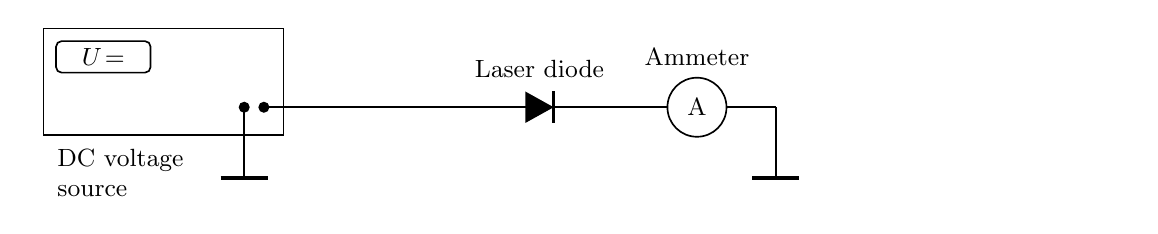
\begin{tikzpicture}[setup]
			\path (-3,0) -- (11,0);
			\pic (src) at (0,0) {instrument={$U\!=$}};
			\node[anchor=north west, align=left] at (-2.75,-0.4) {DC voltage\\source};
			\pic at (src-a) {ground};
			\draw (src-b) -- (6.5,0);
			\pic at (3.5,0) {diode};
			\node[above] at (3.5,0.25) {Laser diode};
			\node[meter] at (5.5,0) {A};
			\node[above] at (5.5,0.4) {Ammeter};
			\pic at (6.5,0) {ground};
		\end{tikzpicture}
		\caption{Current-voltage characteristic.}
		\label{fig:setup_iu}
	\end{subfigure}

	\vspace{0.6cm}
	\begin{subfigure}{\linewidth}
		\centering
		\begin{tikzpicture}[setup]
			\path (-3,0) -- (11,0);
			\pic (gen) at (0,0) {instrument={$I\!=$}};
			\node[anchor=north west, align=left] at (-2.75,-0.4) {Pulse\\generator};
			\pic at (gen-a) {ground};
			\draw (gen-b) -- (5.9,0);
			\draw (0.6,0.15) -- (0.9,0.15) -- (0.9,0.6) -- (1.2,0.6) -- (1.2,0.15) -- (1.5,0.15);
			% voltage measurement at the diode
			\fill (2.2,0) circle (2pt);
			\node[meter] (V) at (2.2,-1.0) {U};
			\draw (2.2,0) -- (V);
			\pic at (V.south) {ground};
			% laser diode on mount with detector
			\pic at (3.6,0) {mount};
			\pic at (3.6,0) {diode};
			\pic at (3.6,0) {emission};
			\draw (4.3,0.8) rectangle (5.5,1.1);
			\node[above] at (4.9,1.1) {Detector};
			\node[meter] at (5.1,0) {A};
			\pic at (5.9,0) {ground};
			% lock-in amplifier
			\pic (lock) at (10.5,0) {instrument={Lock-in}};
			\draw (5.5,0.95) -- (6.8,0.95) -- (6.8,-0.6) -- (10.25,-0.6) -- (lock-a);
			\pic at (lock-b) {ground};
		\end{tikzpicture}
		\caption{Optical power-current characteristic.}
		\label{fig:setup_pi}
	\end{subfigure}

	\vspace{0.6cm}
	\begin{subfigure}{\linewidth}
		\centering
		\begin{tikzpicture}[setup]
			\path (-3,0) -- (11,0);
			\pic (src) at (0,0) {instrument={$I\!=$}};
			\node[anchor=north west, align=left] at (-2.75,-0.4) {DC current\\source};
			\pic at (src-a) {ground};
			\draw (src-b) -- (5.3,0);
			\pic at (3.2,0) {mount};
			\pic at (3.2,0) {diode};
			\pic at (3.2,0) {emission};
			\node[meter] at (4.5,0) {A};
			\pic at (5.3,0) {ground};
			% lens focusing onto the monochromator entrance slit
			\draw (4.0,1.25) ellipse (0.12 and 0.42);
			\draw (4.1,1.6) -- (6.0,1.25) -- (4.1,0.9);
			\draw (6.0,0.6) rectangle (9.2,1.9);
			\node[anchor=south east] at (9.2,0.6) {Monochromator};
			\draw (9.2,1.3) rectangle (10.3,1.9);
			\node at (9.75,1.6) {PMT};
			% computer
			\draw[rounded corners=2pt] (7.9,-1.05) rectangle (9.1,0.05);
			\draw[rounded corners=1pt] (8.05,-0.9) rectangle (8.95,-0.1);
			\draw (8.3,-1.05) -- (8.2,-1.3) -- (8.8,-1.3) -- (8.7,-1.05);
			\draw (7.6,-1.3) rectangle (9.6,-1.85);
			\foreach \x in {7.75,7.85,...,8.45} \draw (\x,-1.42) -- (\x,-1.73);
			\draw (8.9,-1.5) rectangle (9.4,-1.65);
			\draw (9.75,1.3) .. controls (9.9,0.0) and (10.1,-1.4) .. (9.6,-1.55);
		\end{tikzpicture}
		\caption{Spectral measurements.}
		\label{fig:setup_spectral}
	\end{subfigure}
	\caption{Measurement setups for the characterisation of the laser diode. The diode
	is placed on a temperature-controlled mount for the P-I and spectral measurements.
	PMT: photomultiplier tube.}
	\label{fig:setup}
\end{figure}
; reference the whole figure
% with \cref{fig:setup} or a single setup with \cref{fig:setup_iu},
% \cref{fig:setup_pi} and \cref{fig:setup_spectral}.

\tikzset{
	setup/.style={font=\small, line width=0.6pt},
	meter/.style={circle, draw, fill=white, minimum size=0.75cm, inner sep=0pt},
	% instrument box with display; terminals (-a) left and (-b) right, origin at (-b)
	instrument/.pic={
		\draw (-2.8,-0.35) rectangle (0.25,1.0);
		\node[draw, rounded corners=2pt, anchor=north west, minimum width=1.2cm,
			minimum height=0.4cm, inner sep=2pt] at (-2.65,0.85) {#1};
		\fill (-0.25,0) circle (2pt) coordinate (-a);
		\fill (0,0) circle (2pt) coordinate (-b);
	},
	ground/.pic={
		\draw (0,0) -- (0,-0.9);
		\draw[line width=1.4pt] (-0.3,-0.9) -- (0.3,-0.9);
	},
	% laser diode pointing to the right, centred at the origin
	diode/.pic={
		\fill (-0.18,0.2) -- (-0.18,-0.2) -- (0.18,0) -- cycle;
		\draw[line width=1.2pt] (0.18,0.2) -- (0.18,-0.2);
	},
	emission/.pic={
		\draw[-{Stealth[length=4pt]}] (-0.15,0.3) -- (0.2,0.7);
		\draw[-{Stealth[length=4pt]}] (0.05,0.3) -- (0.4,0.7);
	},
	% temperature-controlled mount below the diode
	mount/.pic={
		\draw[fill=gray!30] (-0.12,-0.25) rectangle (0.12,-1.0);
		\draw[fill=gray!60] (-0.3,-1.0) rectangle (0.3,-1.15);
	},
}

\begin{figure}[H]
	\centering
	\begin{subfigure}{\linewidth}
		\centering
		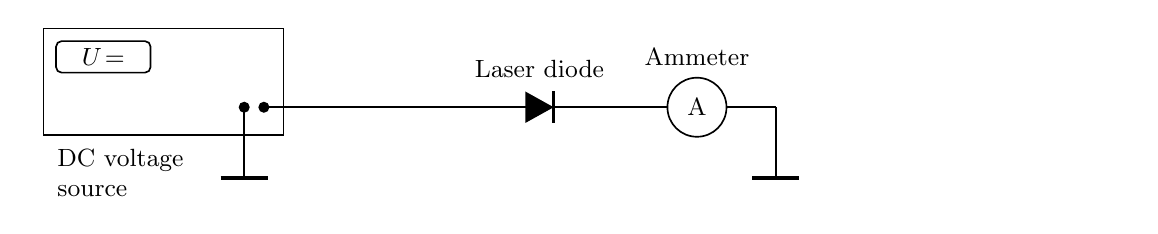
\begin{tikzpicture}[setup]
			\path (-3,0) -- (11,0);
			\pic (src) at (0,0) {instrument={$U\!=$}};
			\node[anchor=north west, align=left] at (-2.75,-0.4) {DC voltage\\source};
			\pic at (src-a) {ground};
			\draw (src-b) -- (6.5,0);
			\pic at (3.5,0) {diode};
			\node[above] at (3.5,0.25) {Laser diode};
			\node[meter] at (5.5,0) {A};
			\node[above] at (5.5,0.4) {Ammeter};
			\pic at (6.5,0) {ground};
		\end{tikzpicture}
		\caption{Current-voltage characteristic.}
		\label{fig:setup_iu}
	\end{subfigure}

	\vspace{0.6cm}
	\begin{subfigure}{\linewidth}
		\centering
		\begin{tikzpicture}[setup]
			\path (-3,0) -- (11,0);
			\pic (gen) at (0,0) {instrument={$I\!=$}};
			\node[anchor=north west, align=left] at (-2.75,-0.4) {Pulse\\generator};
			\pic at (gen-a) {ground};
			\draw (gen-b) -- (5.9,0);
			\draw (0.6,0.15) -- (0.9,0.15) -- (0.9,0.6) -- (1.2,0.6) -- (1.2,0.15) -- (1.5,0.15);
			% voltage measurement at the diode
			\fill (2.2,0) circle (2pt);
			\node[meter] (V) at (2.2,-1.0) {U};
			\draw (2.2,0) -- (V);
			\pic at (V.south) {ground};
			% laser diode on mount with detector
			\pic at (3.6,0) {mount};
			\pic at (3.6,0) {diode};
			\pic at (3.6,0) {emission};
			\draw (4.3,0.8) rectangle (5.5,1.1);
			\node[above] at (4.9,1.1) {Detector};
			\node[meter] at (5.1,0) {A};
			\pic at (5.9,0) {ground};
			% lock-in amplifier
			\pic (lock) at (10.5,0) {instrument={Lock-in}};
			\draw (5.5,0.95) -- (6.8,0.95) -- (6.8,-0.6) -- (10.25,-0.6) -- (lock-a);
			\pic at (lock-b) {ground};
		\end{tikzpicture}
		\caption{Optical power-current characteristic.}
		\label{fig:setup_pi}
	\end{subfigure}

	\vspace{0.6cm}
	\begin{subfigure}{\linewidth}
		\centering
		\begin{tikzpicture}[setup]
			\path (-3,0) -- (11,0);
			\pic (src) at (0,0) {instrument={$I\!=$}};
			\node[anchor=north west, align=left] at (-2.75,-0.4) {DC current\\source};
			\pic at (src-a) {ground};
			\draw (src-b) -- (5.3,0);
			\pic at (3.2,0) {mount};
			\pic at (3.2,0) {diode};
			\pic at (3.2,0) {emission};
			\node[meter] at (4.5,0) {A};
			\pic at (5.3,0) {ground};
			% lens focusing onto the monochromator entrance slit
			\draw (4.0,1.25) ellipse (0.12 and 0.42);
			\draw (4.1,1.6) -- (6.0,1.25) -- (4.1,0.9);
			\draw (6.0,0.6) rectangle (9.2,1.9);
			\node[anchor=south east] at (9.2,0.6) {Monochromator};
			\draw (9.2,1.3) rectangle (10.3,1.9);
			\node at (9.75,1.6) {PMT};
			% computer
			\draw[rounded corners=2pt] (7.9,-1.05) rectangle (9.1,0.05);
			\draw[rounded corners=1pt] (8.05,-0.9) rectangle (8.95,-0.1);
			\draw (8.3,-1.05) -- (8.2,-1.3) -- (8.8,-1.3) -- (8.7,-1.05);
			\draw (7.6,-1.3) rectangle (9.6,-1.85);
			\foreach \x in {7.75,7.85,...,8.45} \draw (\x,-1.42) -- (\x,-1.73);
			\draw (8.9,-1.5) rectangle (9.4,-1.65);
			\draw (9.75,1.3) .. controls (9.9,0.0) and (10.1,-1.4) .. (9.6,-1.55);
		\end{tikzpicture}
		\caption{Spectral measurements.}
		\label{fig:setup_spectral}
	\end{subfigure}
	\caption{Measurement setups for the characterisation of the laser diode. The diode
	is placed on a temperature-controlled mount for the P-I and spectral measurements.
	PMT: photomultiplier tube.}
	\label{fig:setup}
\end{figure}
; reference the whole figure
% with \cref{fig:setup} or a single setup with \cref{fig:setup_iu},
% \cref{fig:setup_pi} and \cref{fig:setup_spectral}.

\tikzset{
	setup/.style={font=\small, line width=0.6pt},
	meter/.style={circle, draw, fill=white, minimum size=0.75cm, inner sep=0pt},
	% instrument box with display; terminals (-a) left and (-b) right, origin at (-b)
	instrument/.pic={
		\draw (-2.8,-0.35) rectangle (0.25,1.0);
		\node[draw, rounded corners=2pt, anchor=north west, minimum width=1.2cm,
			minimum height=0.4cm, inner sep=2pt] at (-2.65,0.85) {#1};
		\fill (-0.25,0) circle (2pt) coordinate (-a);
		\fill (0,0) circle (2pt) coordinate (-b);
	},
	ground/.pic={
		\draw (0,0) -- (0,-0.9);
		\draw[line width=1.4pt] (-0.3,-0.9) -- (0.3,-0.9);
	},
	% laser diode pointing to the right, centred at the origin
	diode/.pic={
		\fill (-0.18,0.2) -- (-0.18,-0.2) -- (0.18,0) -- cycle;
		\draw[line width=1.2pt] (0.18,0.2) -- (0.18,-0.2);
	},
	emission/.pic={
		\draw[-{Stealth[length=4pt]}] (-0.15,0.3) -- (0.2,0.7);
		\draw[-{Stealth[length=4pt]}] (0.05,0.3) -- (0.4,0.7);
	},
	% temperature-controlled mount below the diode
	mount/.pic={
		\draw[fill=gray!30] (-0.12,-0.25) rectangle (0.12,-1.0);
		\draw[fill=gray!60] (-0.3,-1.0) rectangle (0.3,-1.15);
	},
}

\begin{figure}[H]
	\centering
	\begin{subfigure}{\linewidth}
		\centering
		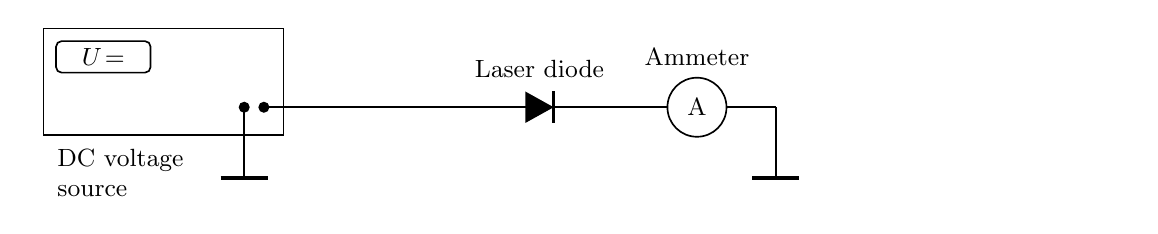
\begin{tikzpicture}[setup]
			\path (-3,0) -- (11,0);
			\pic (src) at (0,0) {instrument={$U\!=$}};
			\node[anchor=north west, align=left] at (-2.75,-0.4) {DC voltage\\source};
			\pic at (src-a) {ground};
			\draw (src-b) -- (6.5,0);
			\pic at (3.5,0) {diode};
			\node[above] at (3.5,0.25) {Laser diode};
			\node[meter] at (5.5,0) {A};
			\node[above] at (5.5,0.4) {Ammeter};
			\pic at (6.5,0) {ground};
		\end{tikzpicture}
		\caption{Current-voltage characteristic.}
		\label{fig:setup_iu}
	\end{subfigure}

	\vspace{0.6cm}
	\begin{subfigure}{\linewidth}
		\centering
		\begin{tikzpicture}[setup]
			\path (-3,0) -- (11,0);
			\pic (gen) at (0,0) {instrument={$I\!=$}};
			\node[anchor=north west, align=left] at (-2.75,-0.4) {Pulse\\generator};
			\pic at (gen-a) {ground};
			\draw (gen-b) -- (5.9,0);
			\draw (0.6,0.15) -- (0.9,0.15) -- (0.9,0.6) -- (1.2,0.6) -- (1.2,0.15) -- (1.5,0.15);
			% voltage measurement at the diode
			\fill (2.2,0) circle (2pt);
			\node[meter] (V) at (2.2,-1.0) {U};
			\draw (2.2,0) -- (V);
			\pic at (V.south) {ground};
			% laser diode on mount with detector
			\pic at (3.6,0) {mount};
			\pic at (3.6,0) {diode};
			\pic at (3.6,0) {emission};
			\draw (4.3,0.8) rectangle (5.5,1.1);
			\node[above] at (4.9,1.1) {Detector};
			\node[meter] at (5.1,0) {A};
			\pic at (5.9,0) {ground};
			% lock-in amplifier
			\pic (lock) at (10.5,0) {instrument={Lock-in}};
			\draw (5.5,0.95) -- (6.8,0.95) -- (6.8,-0.6) -- (10.25,-0.6) -- (lock-a);
			\pic at (lock-b) {ground};
		\end{tikzpicture}
		\caption{Optical power-current characteristic.}
		\label{fig:setup_pi}
	\end{subfigure}

	\vspace{0.6cm}
	\begin{subfigure}{\linewidth}
		\centering
		\begin{tikzpicture}[setup]
			\path (-3,0) -- (11,0);
			\pic (src) at (0,0) {instrument={$I\!=$}};
			\node[anchor=north west, align=left] at (-2.75,-0.4) {DC current\\source};
			\pic at (src-a) {ground};
			\draw (src-b) -- (5.3,0);
			\pic at (3.2,0) {mount};
			\pic at (3.2,0) {diode};
			\pic at (3.2,0) {emission};
			\node[meter] at (4.5,0) {A};
			\pic at (5.3,0) {ground};
			% lens focusing onto the monochromator entrance slit
			\draw (4.0,1.25) ellipse (0.12 and 0.42);
			\draw (4.1,1.6) -- (6.0,1.25) -- (4.1,0.9);
			\draw (6.0,0.6) rectangle (9.2,1.9);
			\node[anchor=south east] at (9.2,0.6) {Monochromator};
			\draw (9.2,1.3) rectangle (10.3,1.9);
			\node at (9.75,1.6) {PMT};
			% computer
			\draw[rounded corners=2pt] (7.9,-1.05) rectangle (9.1,0.05);
			\draw[rounded corners=1pt] (8.05,-0.9) rectangle (8.95,-0.1);
			\draw (8.3,-1.05) -- (8.2,-1.3) -- (8.8,-1.3) -- (8.7,-1.05);
			\draw (7.6,-1.3) rectangle (9.6,-1.85);
			\foreach \x in {7.75,7.85,...,8.45} \draw (\x,-1.42) -- (\x,-1.73);
			\draw (8.9,-1.5) rectangle (9.4,-1.65);
			\draw (9.75,1.3) .. controls (9.9,0.0) and (10.1,-1.4) .. (9.6,-1.55);
		\end{tikzpicture}
		\caption{Spectral measurements.}
		\label{fig:setup_spectral}
	\end{subfigure}
	\caption{Measurement setups for the characterisation of the laser diode. The diode
	is placed on a temperature-controlled mount for the P-I and spectral measurements.
	PMT: photomultiplier tube.}
	\label{fig:setup}
\end{figure}
